\documentclass[12pt]{article}

\usepackage[table]{xcolor}

\usepackage[hidelinks]{hyperref}
\usepackage{etoolbox}
\usepackage{graphicx}
\usepackage{adjustbox}

\makeatletter
\def\ScaleIfNeeded{%
  \ifdim\Gin@nat@width>\linewidth
    \linewidth
  \else
    \Gin@nat@width
  \fi
}
\makeatother

% fonts
\usepackage[T1]{fontenc}
\usepackage[utf8]{inputenc}
\usepackage{textgreek}
\usepackage[greek,english]{babel}
\usepackage{amsmath}

% Code highlight and colors
\usepackage{listings}
\lstset{
  numbers=left,
  tabsize=1,
  basicstyle=\small\ttfamily,
  breaklines=true
}

\usepackage{booktabs, tabularx, longtable}
\usepackage{csquotes}
\usepackage{authblk}

% Geometry block
\usepackage[letterpaper]{geometry}
\providecommand{\tightlist}{\setlength{\itemsep}{0pt}\setlength{\parskip}{0pt}}

\title{Complex Ecological Networks}

\author[1,2]{Mathilde~Besson}
\author[1,2]{Eva~Delmas*}
\author[1,2]{Timothée~Poisot}
\author[2,3]{Dominique~Gravel}
\affil[1]{Université de Montréal, Département de Sciences Biologiques}
\affil[2]{Québec Centre for Biodiversity Sciences}
\affil[3]{Université de Sherbrooke, Département de Biologie}

\begin{document}

\maketitle

\begin{abstract}
  Introduction to ecological network
\end{abstract}

% pandoc-xnos: macro to create a caption without a prefix
\makeatletter
\long\def\@makenoprefixcaption#1#2{
  \vskip\abovecaptionskip
  \sbox\@tempboxa{#2}
  \ifdim \wd\@tempboxa >\hsize
    #2\par
  \else
    \global \@minipagefalse
    \hb@xt@\hsize{\hfil\box\@tempboxa\hfil}
  \fi
  \vskip\belowcaptionskip}
\makeatother

% pandoc-fignos: save original macros
\makeatletter
\let\@oldmakecaption=\@makecaption
\let\oldthefigure=\thefigure
\let\oldtheHfigure=\theHfigure
\makeatother

% pandoc-fignos: environment disables figure caption prefixes
\makeatletter
\newcounter{figno}
\newenvironment{no-prefix-figure-caption}{
  \let\@makecaption=\@makenoprefixcaption
  \renewcommand\thefigure{x.\thefigno}
  \renewcommand\theHfigure{x.\thefigno}
  \stepcounter{figno}
}{
  \let\thefigure=\oldthefigure
  \let\theHfigure=\oldtheHfigure
  \let\@makecaption=\@oldmakecaption
  \addtocounter{figure}{-1}
}
\makeatother

% pandoc-xnos: cleveref fakery
\newcommand{\plusnamesingular}{}
\newcommand{\starnamesingular}{}
\newcommand{\xrefname}[1]{\protect\renewcommand{\plusnamesingular}{#1}}
\newcommand{\Xrefname}[1]{\protect\renewcommand{\starnamesingular}{#1}}
\providecommand{\cref}{\plusnamesingular~\ref}
\providecommand{\Cref}{\starnamesingular~\ref}
\providecommand{\crefformat}[2]{}
\providecommand{\Crefformat}[2]{}

% pandoc-xnos: cleveref formatting
\crefformat{figure}{fig.~#2#1#3}
\Crefformat{figure}{Figure~#2#1#3}
\crefformat{table}{table~#2#1#3}
\Crefformat{table}{Table~#2#1#3}
\crefformat{equation}{eq.~#2#1#3}
\Crefformat{equation}{Equation~#2#1#3}

\section{Glossary}\label{glossary}

Adjacency matrix: square matrix representing species interactions. If
two species \(i\) and \(j\) interact, the intersection of the matrix at
\({i,j}\) will be 1, and if no interaction.

Assembly rules: Ecological processes that lead to a specific species'
composition of a community, \emph{e.g.} competition, predator-prey
interactions, arrival history, etc.

\textbf{Bipartite / Unipartite network} The entire representation of the
adjacency matrix offers an \emph{unipartite} network representation,
where the hierarchy between nodes and their position into the network is
not always visible (\emph{Figure 1}). On the contrary, a bipartite or
k-partite network is a hierarchical representation of the network
(\emph{Figure 2}), where nodes are separated depending on their position
or function into the network (\emph{e.g} pollinator-plant as bipartite
network).

Ecological interactions: Every type of contact between two species that
alters the abundance, biomass and/or behavior of one or both species.
Interactions can be trophic, mutualistic or antagonistic, directed or
undirected, weighted or unweighted.

Ecosystem functioning: Biotic and abiotic processes that regulate
ecosystem, allowing energy and matter flux between trophic levels and
between ecosystems, \emph{e.g.} biogeochemical cycles.

Graph theory: Mathematical framework used to model the relationship
between the objects of a network

Network structure: General shape of a network. It is commonly measured
using connectance, link distribution, general architecture (nestedness
and modularity), etc.

Nodes/Links, Vertices/Edges: Following graph theory, species are
represented as nodes (or vertices), and interactions between them are
represented by links (or edges).

Phylogenetic signal: tendency of phylogenetically close species to have
similar traits.

\section{Nomenclature}\label{nomenclature}

\(N\) population size

\(r\) growth rate

\(A\) adjacency matrix

\(\alpha\) interaction strength

\section{}\label{section}

\subsection{Introduction}\label{introduction}

In ecological systems (\emph{e.g.} communities), interactions between
components (\emph{e.g.} species) are organized in ways that are
non-random and constrained by sets of rules (see section X). The
organization of these interactions drives or changes some properties of
the community, such as its stability, productivity, or ability to resist
extinctions, which eventually feedback on the system organization. This
constant interplay between interaction organization and system functions
results in signatures on the system structure (\emph{e.g.} invariance in
key features of the system structure, see section X). Detecting and
analyzing these signatures gives us information on the system itself.
Studying the structure of ecological systems is necessary to gain
insights on the fundamental rules and processes that govern ecosystem
formation, maintenance and functioning.

The way interactions are organized can be studied by investigating the
structure of ecological networks. Designed to analyze the structure of a
studied system, the \emph{graph theory} is a mathematical framework
which seemed to be largely appropriate to answer ecological questions.
Every system can be abstracted by a \emph{graph}, a representation of
the system components organization (\emph{Figure 1a}). These components
are called \emph{nodes} and are linked together by \emph{edges}. These
combinations form the structure of the studied system. In an ecological
system, nodes can be individuals, populations, communities or landscape
patches and edges can represent trophic links, energetic flux, etc,
every kind of interaction. Both nodes and edges can carry additional
information such as weight (\emph{e.g.} species abundance, intensity of
the gene flow between two populations, etc.), location in space and
time, edges direction and sign and nodes labels (\emph{e.g.} species
identity). Specific informations can be attached to edges, modifying the
characteristics of the graph. Graphs can be \emph{directed} (\emph{i.e}
interaction goes from A to B) or \emph{undirected}, \emph{weighted}
(\emph{i.e} different strength of interaction among the network) or
\emph{unweighted} (\emph{Figures 1 and 2}). This information is
summarized mathematically in the \emph{adjacency matrix} (typically
named \(A\), see definition in glossary) (\emph{Figure 1b}). In this
paper, for simplicity, time and space, we decided to mostly focus on
\emph{Species Interaction Networks} (SIN). Ecological system such as
landscape, genetic or nutrient networks are not represented here, but
they can be studying following the same framework defined further
{[}\emph{ref}{]}.

Describing and understanding the structure of species interaction
networks is an active, and growing, field of ecological research. In
this contribution, we will give an overview of some of the most
prominent findings and areas of research from the last decade. Starting
from a discussion of some invariant properties of the structure of
species interaction networks, we will then discuss how this structure
affects ecological properties. We will follow by a discussion of the
ways ecological networks can be studied under familiar concepts from
ecological theory, and finally how this approach scales up to larger
temporal or spatial scales.

\begin{no-prefix-figure-caption}

\begin{figure}
\centering
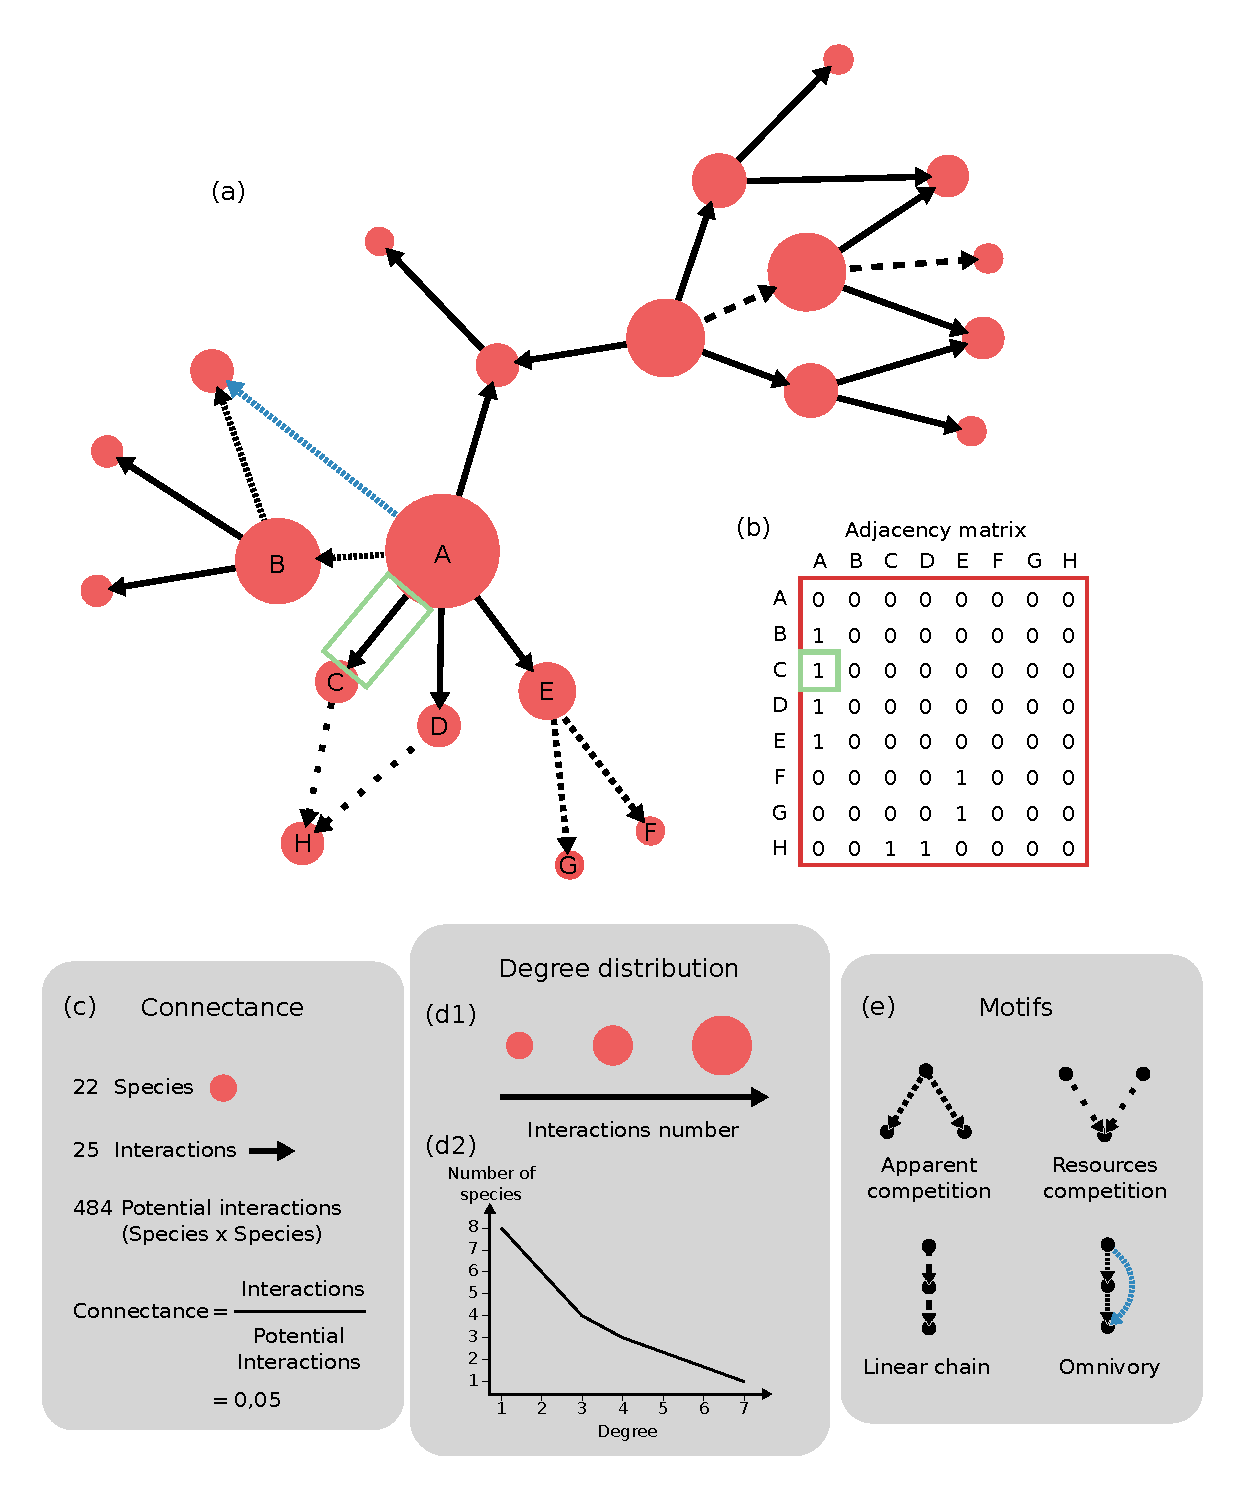
\includegraphics[width=1.00000\textwidth]{Figures/figure1.pdf}
\caption{Figure 1: Graphical representation of a fictional ecological
network (a), where species are represented by circles and their directed
interactions by arrows. The representation is build from the adjacency
matrix (b). In an unipartite representation as this one, each species is
represented both as a column and a row. 1 indicates an interaction
between two species (e.g.~the green square in (b)), and 0 indicates the
absence of interaction. This matrix allows to calculate network
characteristics such as the connectance (c) and the degree distribution
(d). (c) represents the level of connection into the network and is
calculated as shown in the figure. (d) represents the distribution of
interaction per species. The circles size is relative to the amount of
interactions a species have (d1). This distribution is non-random and
generally follows a power-law distribution (d2). The network can be
split into subnets composed of 3 species, called motif (e). Among the 13
different possible motifs, we only represented the most commonly found
in natural communities.}
\end{figure}

\end{no-prefix-figure-caption}

\subsection{Invariants in ecological
networks}\label{invariants-in-ecological-networks}

One striking particularity of ecological networks is their consistency:
even though they depict interactions between different organisms across
all sorts of ecosystems, they all tend to look the same (Jordano,
Bascompte and Olesen, 2003). Remarkably, even when interactions among
species themselves vary (see section \textbf{x}), the overall network
structure tends to remain unchanged (Kemp, Evans, Augustyn and Ellis,
2017). Most ecological networks have a very specific degree distribution
(Williams, 2011) (\emph{Figure 1d}), whereby most species have a small
number of interactions, and a small proportions of species have a large
number of interactions. In food webs, which represent interactions
between preys and their predators, there is a well-described
relationship between the number of species and the number of
interactions: the number of interactions (\(L\)) increases
proportionally to the number of species (\(S\)) raised to some exponent,
or \(L \propto S^k\). Martinez (1992) suggested that this exponent is
approximately equal to 2, \emph{i.e.} the number of interactions is
proportional to the squared number of species. Brose, Ostling, Harrison
and Martinez (2004) show that this general relationship holds even
across space: it is possible to estimate how many interactions a species
will establish across its entire range. In some other instances,
networks may differ on some aspect of their structure, despite obeying
to a shared underlying principle. For example, Fortuna, Stouffer and
Olesen \emph{et al.} (2010) show that in networks with a low connectance
(\emph{Figure 1c}), nestedness (the degree to which the diet of
specialists and generalists overlaps -- \emph{Figure 2}) and modularity
(the tendency of species to form densely aggregated clusters --
\emph{Figure 2}) are positively correlated. In networks with higher
connectance, this became the opposite: networks with a large number of
interactions were either nested (and not modular) or modular (and not
nested). In the recent years, it emerged that many aspects of network
structure covary with connectance (Poisot and Gravel, 2014; Chagnon,
2015): this suggests that simply knowing how many species there are, and
how many interactions they establish, is already very informative about
the network structure.

\begin{no-prefix-figure-caption}

\begin{figure}
\centering
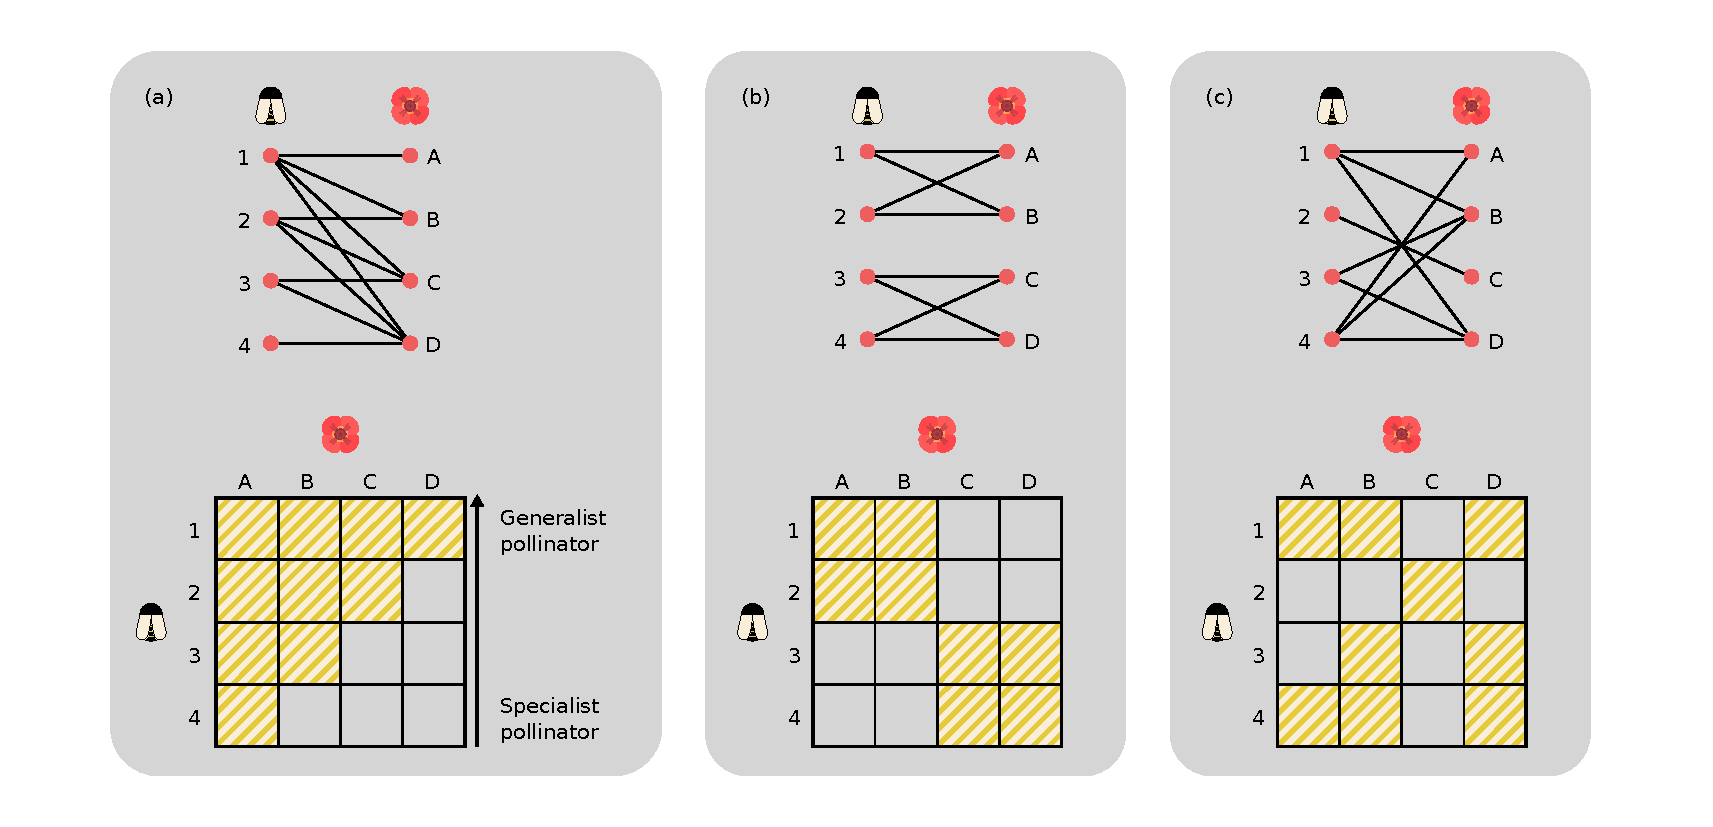
\includegraphics[width=1.00000\textwidth]{Figures/figure2.pdf}
\caption{Figure 2: Network topology, example of a fictional
plant-pollinator network. (a) shows a perfectly nested network, where
specialists pollinators are visiting plants embedded into the diet of
more generalist pollinators. (b) shows a perfectly modular network,
where sub-groups of species interact more strongly with each over than
with the rest of the network. (c) shows a random network. Two
representations are possibles. Top: Bipartite representation using nodes
and edges ; Bottom: Ordered interaction matrix. Here, we used striped
yellow squares instead of 1 for presence of interaction and empty
squares in absence of interaction.}
\end{figure}

\end{no-prefix-figure-caption}

Another remarkable generality of network structure is the distribution
of particular shapes of interconnection between three-species subsets.
Milo (2002) found that networks (not just ecological but other types of
networks such as neuronal or electronical networks as well) can be
characterized by the over or under representation of some of these
three-species subset, which they called motifs (\emph{Figure 1e}).
Motifs can be more broadly defined as being particular shapes of
interconnection between three or more nodes in networks at a frequency
significantly higher than those found in randomized networks.
Three-species motifs represent the simplest building blocks of networks,
and more importantly the typical interaction found in communities. As
such, they offer the possibility to integrate and test theories
developed on simple modules (\emph{e.g.} omnivory, McCann, Hastings and
Huxel (1998), Holt (1997)) in larger, more realistic networks. Food
webs, for example, are characterized by an over representation of linear
food chains and omnivory and an under representation of apparent and
exploitative competition (Bascompte and Melián, 2005; Camacho, Stouffer
and Amaral, 2007). Stouffer and Bascompte (2010) found that this
distribution promotes stability in food webs, with over-represented
motifs being more stable in isolation and correlated with higher
stability in large realistic communities, and conversely. Motifs can
also be used to characterize species role in networks. From the 13
different three-species motifs emerge 30 unique positions for species to
occupy in these motifs, representing how the species is embedded in its
community. The different positions a species will occupy, and the
frequency with which it will occupy these different positions in
networks are called species motif role (Stouffer, Sales-Pardo, Sirer and
Bascompte, 2012). These roles have been shown to be evolutionary
conserved in food webs (Stouffer, Sales-Pardo, Sirer and Bascompte,
2012) and to have less variability in time than expected in
host-parasitoids bipartite networks (Baker, Kaartinen, Roslin and
Stouffer, 2015).

Another invariant network property lies in species phylogeny. Phylogeny
is a key determinant of ecological network structure, allowing the
understanding of species position and interactions into the community.
Phylogenetically close species indeed inherit traits from their common
ancestors (\emph{e.g.} body size, habitat, defensive strategy, metabolic
type, phenology), increasing their propensity to interact with the same
group of species or with similar species. This conservatism of
interactions has been found to hold across different types of
interactions such as antagonistic or mutualistic interactions (Fontaine
and Thébault, 2015). However, every species role, such as host or
parasite in antagonistic interaction, prey or predator in food web and
plant or pollinator/seed disperser in mutualistic interaction, do not
provide the same links structure. For instance, closely related host
tend to share parasites, while closely related parasites, because of
competition for resources, tend to have different hosts species
(Krasnov, Fortuna and Mouillot \emph{et al.}, 2012). The conservatism of
interactions is consequently unequal all over the network. Following the
logic that closely related species interact with the same group of
species, Rezende, Albert, Fortuna and Bascompte (2009) shown that
phylogenetic structure of ecological networks explains almost entirely
the formation and composition of modules in the network, and the
connections between them. For the same reasons that conservatism of
interactions is asymmetrical, the link between phylogenetic signal and
module composition is different depending on the species role (Krasnov,
Fortuna and Mouillot \emph{et al.}, 2012), and species that are modules
connector are usually phylogenetically close. Cattin, Bersier and
Banašek-Richter \emph{et al.} (2004) also found, using a
niche-hierarchic model, that diet is constrained by the phylogenetic
origin of consumers. The nested structure of trophic networks, generated
by the diet structuration, is then influenced by the phylogenetic signal
of interacting species and the compatibility of their traits. In
contrast, the nested structure of mutualistic networks would be a
consequence of trait complementary between species (Rezende, Jordano and
Bascompte, 2007). For now, mechanisms underlying the
nestedness-phylogeny relationship remain to be further investigated.
Moreover, because of species plasticity, phylogeny alone does not fully
the structure and evolution of ecological networks.

\subsection{From structure to
properties}\label{from-structure-to-properties}

The relationship between ecological network structure and stability
remains a contemporary topic of discussion. First, MacArthur (1955) and
Elton (1958) observed in natural ecosystems that diverse communities
have a more stable dynamic than simple ones. Using a mathematical model
based on random ecological networks, May (1972) undermined this
hypothesis. Taking into account not only species diversity but also the
connectance and the interaction strengths in the network, he found that,
contrarily to the way of thinking at this time, diversity was
destabilizing communities. This kick in the anthill was the beginning of
a prolific complexity-stability debate, highly oriented on trophic
networks (McCann, 2000; see Allesina and Tang, 2015). Two different
approaches of the stability have emerged: one based on the general
complexity-stability relationship and dynamics among species in
communities and the second one based on the communities ability to
resist biotic and abiotic changes. The both use different notions and
definitions of stability, inducing different ways to study it (see
{\textbf{???}}). Despite their dissimilarities, these approaches are not
totally independent and have allowed highlighting that species diversity
has no direct influence on communities stability. However, the structure
of ecological network such as interactions distribution and strength
seems to play a crucial role (Yodzis, 1981). The links distribution of
ecological networks follows a power-law distribution (Montoya and Solé,
2002), meaning that few species are highly connected to the rest of the
community and a large number of species are weakly connected to others.
This organization combined with the myriad of weak interactions found
across ecological networks, called the weak interaction effect (Berlow,
1999), buffers species variations and then stabilizes the entire
community (Bascompte, Melián and Sala, 2005; Jacquet, Moritz and
Morissette \emph{et al.}, 2016). Other parameters, such as the
predator-prey body-mass ratio (Emmerson and Raffaelli, 2004; Brose,
Jonsson and Berlow \emph{et al.}, 2006) or network architecture
(Montoya, Pimm and Solé, 2006; Thébault and Fontaine, 2010), determine
the distribution and strength of interactions and then contribute to the
stability of ecological networks.

Perturbations in ecological communities, generally caused by landscape
fragmentation, habitat loss, species loss or invasion, induce a decrease
of species diversity. This loss of diversity is explained by extinctions
of species due directly or indirectly to a first species loss
(\emph{i.e.} secondary extinctions or cascade of extinctions). These
extinctions are used to measure the robustness of ecological communities
and to explore what happen when a species is removed or changed in a
network. The use of dynamic-based models led to highlight the fact that
the probability of secondary extinctions increases with the community
size (Lundberg, Ranta and Kaitala, 2008), and decreases with the network
connectance (Dunne, Williams and Martinez, 2002). Then, the focus on
species removal have allowed to understand that the loss of an highly
connected species, also called hub, induces a higher rate of secondary
extinctions than the loss of a random, weakly connected species (Solé
and Montoya, 2001). However, even if a species is weakly directly
connected, if it represents a highway of energy-flow in the network
(carbon, nitrogen or biomass), its loss will have similar impact in term
of secondary extinctions than the loss of an hug (Allesina and Bodini,
2004). The network architecture also affects the community response to
perturbations. For instance, thanks to their structural properties
(hight nestedness and connectance, Jordano, Bascompte and Olesen
(2003)), mutualistic networks persist longer than randomly structured
networks (Memmott, Waser and Price, 2004 ; Fortuna and Bascompte, 2006).
On the other hand, presence of modules in the community structure limits
propagation of perturbations across the rest of the network and then
secondary extinctions (Stouffer and Bascompte, 2010).

The consequences of the erosion of biodiversity for ecosystem
functioning has been for almost three decades a central problematic for
ecologists. While the hypothesis that an increase in species diversity
results in an increased productivity dates back to Darwin (Darwin,
1859), the emergence of experimental ecology and the shift from
observation in natural systems to the quantification of ecology has made
possible to develop a quite general theory for what is now called the
biodiversity-ecosystem functioning (BEF) relationship. In a trophic
group (\emph{i.e.} a group of species that all belong to the same
trophic level, \emph{e.g.} producers or herbivores), the loss of
diversity results in a loss of efficiency to capture the shared resource
compartment (Loreau, 2010) (\emph{e.g.} nutrients for producers, or
producers for herbivores). This leading to a decrease in productivity or
other index of functioning. Yet, when the trophic group under focus is
coupled to other(s), the action of diversity on functioning is more
variable (Duffy, Cardinale and France \emph{et al.}, 2007). This makes
the BEF relationship unpredictable in real-world communities, composed
of several trophic groups that are virtually never differentiable -- as
intraguild predation and omnivory blurr the frontier between levels. The
multiplicity of the factors influencing the BEF relationship calls for a
more general framework that allows the integration of the theories
developped for trophic group and for simple modules or sub-systems. By
mapping transfer of biomass and energy and/or constraints on organism
through the different compartments that compose a natural community,
ecological networks -- and food webs in particular -- offer the
possibility to perform this integration. Analyses performed on simulated
food-webs with unchanged diversity have already shown that interactions,
and more specifically their structure, have a significative influence on
functioning (Thebault and Loreau, 2003; Thébault, Huber and Loreau,
2007; Poisot, Mouquet and Gravel, 2013). The structure of interactions
translates the distribution of different types of properties important
for ecosystem functioning, such as the presence of omnivory, the
generality of species, the modularity of the food-web, etc.

\subsection{Linking interactions to ecological
mechanisms}\label{linking-interactions-to-ecological-mechanisms}

It is worth remembering that ecological interactions are the direct
expression of ecological mechanisms. A pollinator is able to effectively
reach the nectar in a plant because the traits of the two organisms
match, because they have compatible phenologies, and because they occur
in the same environment. A virus can infect its host because it is able
to attach to the cell surface, effectively penetrate it, and hijack the
cellular machinery to its benefit. Interactions that are not allowed
because trait values do not match have been called \enquote{forbidden
links} (Olesen, Bascompte and Dupont \emph{et al.}, 2011). This prompted
a search for \enquote{linkage rules} (Bartomeus, 2013) in ecological
networks, \emph{i.e.} the relationships that must exist between traits
borne by two organisms in order for an interaction between them to
exist. These can be identified from existing data on traits and
interactions (Bartomeus, Gravel and Tylianakis \emph{et al.}, 2016), and
then used to generate realistic ecological networks (Crea, Ali and
Rader, 2015). González-Varo and Traveset (2016) point out that
interactions are happening between individuals: this requires to
consider how the traits are distributed at the individual scale, but
also how different behaviors may allow organisms to overcome some of the
forbidden links. Although traits are an important part of what makes
interactions happen, they are only relevant insofar as the organisms are
able to encounter one another. The importance of neutral dynamics
(\emph{i.e.} how abundances of different species can determine the
probability that they can interact, based on how often they would bump
into one another by chance) is, somewhat counter-intuitively, great.
Canard, Mouquet and Marescot \emph{et al.} (2012) reveals that
simulating food web dynamics by using only population abundances to
predict interactions yields realistic food webs. In a host-parasite
system, local abundances has also been identified as a key predictor of
species interactions (Canard, Mouquet and Mouillot \emph{et al.}, 2014).
Speaking more broadly, because interactions emerge from all of these
ecological mechanisms, there is a need to develop a deeper understanding
of their variability (Poisot, Stouffer and Gravel, 2015). Beyond the
fundamental advance that this represents, this would allow to predict
interactions based on external information (Morales-Castilla, Matias,
Gravel and Araújo, 2015).

The realization of an interaction between individuals from the same or
different populations within a community also have ecological
consequences as it modifies the dynamics of at least one of the
interacting populations, and through it, emerging properties. If we
consider for instance a population A, its dynamics is not the same when
it multiplies in isolation -- where it can grow exponentially if
resources are unlimited (Malthus, 1798) or logistically otherwise
(Verhulst, 1938) -- or when it is embedded in a real-world community,
composed of several species interacting with one another through
different mechanisms (Chesson and Kuang, 2008). It can lose individuals
to predation, have parasitism increase its death rate and at the same
time see its establishment eased through facilitation. It then becomes
necessary to account for interactions when studying the dynamic a
population, community stability or ecosystem functioning. But the effect
of interactions on populations dynamics is not always straightforward,
both in terms of directionality and intensity, as there is different
types of interactions and multiple factors influence their probability
of occurrence and strength. Since the seminal work of May (1972), the
analysis of these effects has been a prolific field of ecology, feeding
in particular the famous \enquote{complexity-stability debate} (see
Allesina and Tang (2015) for an overview). Including interactions in
population dynamics analyses can be done by using model of the following
general form:

\[
\frac{1}{N_i}\frac{\text{d}}{\text{d}t}N_i = r_i \times \sum_j A_{ij} \alpha_{i,j} N_j \,
\]

wherein the adjacency matrix \(A\) (\(n*n\)), list the realized
interactions in a given community composed of \(n\) species.
\(A_{ij} \neq 0\) when species \(i\) and \(j\) interact and \(0\)
otherwise. \(\alpha_{ij}\) quantifies the strength of the interaction.
This equation model populations abundance \(N\) but can easily be
adapted to model biomass flows by replacing populations' abundances by
their biomasses \(B_i\) (see for instance Williams, Brose and Martinez
(2007)).

Ecological networks are also spatially and temporally variable
(Trøjelsgaard and Olesen, 2016). There are two drivers to this
variability: changes in species composition, and changes in the way
these species interact (Poisot, Canard and Mouillot \emph{et al.},
2012). Changes in species alone are able to generate variation in
network properties (Havens, 1992). Spatial variation in network
structure can also reflect deep-time constraints; for example,
Dalsgaard, Trøjelsgaard and Martín González \emph{et al.} (2013) reveal
that historical climate change trends have a signature on the nestedness
and modularity of pollination networks. Even when the same species are
present, interactions between them can vary. Carstensen, Sabatino,
Trøjelsgaard and Morellato (2014) and Trøjelsgaard, Jordano, Carstensen
and Olesen (2015) investigated this phenomenon in mutualistic networks.
Interaction turnover results from variations in partner fidelity (some
species pairs are extremely closely associated), but also from
variations in the local environment in which the species interact.
Interestingly, and as mentioned in section \textbf{x}, networks
overwhelmingly tend to conserve their structure even when interactions
within them change. Díaz-Castelazo, Guimarães and Jordano \emph{et al.}
(2010) surveyed a pollination network over 10 years, and found important
species turnover during this period. Nevertheless, the network retained
its structure because species where replaced by their functional
equivalent; a generalist pollinator often succeeded to another
generalist pollinator. Conversely, species tend to retain their role in
different communities: Baker, Kaartinen, Roslin and Stouffer (2015) show
that species keep occupying the same position in the network across
space, regardless of the species they interact with at every location.

\subsection{From the regional species pool to local structured
communities}\label{from-the-regional-species-pool-to-local-structured-communities}

Describing the different local communities that occur at macroecological
scales through their ecological networks represent an additional layer
of information compared to simple species lists. As such, ecological
networks are a powerful tool to shed new light on the processes
underlying species distribution (Cazelles, Araújo, Mouquet and Gravel,
2016). Until recently, the prevailing idea was that at large scales, the
role of biotic interactions was very small compared to that of abiotic
conditions, and thought to only be important locally (Pearson and
Dawson, 2003; Boulangeat, Gravel and Thuiller, 2012). Empirical
observations of species-environment relationship are then used to
understand species physiological tolerance to environmental conditions
and potentially predict their range under different scenarios of climate
change (e.g. Araújo, Thuiller and Pearson, 2006). While these climate
envelope models provide a useful approximation of species potential
distribution (Pearson, Dawson, Berry and Harrison, 2002), there is
mounting evidences that biotic interactions -- both positive and
negative -- play a critical role in shaping communities not only at
local scales (Boulangeat, Gravel and Thuiller, 2012), but also at
macroecological scales (Davis, Lawton, Shorrocks and Jenkinson, 1998;
Araújo and Luoto, 2007; Heikkinen, Luoto and Virkkala \emph{et al.},
2007; Gotelli, Graves and Rahbek, 2010; Araújo, Rozenfeld, Rahbek and
Marquet, 2011). So far, the role of interactions in shaping species
distribution is mainly estimated from co-occurrence data, used to build
joint species distribution models (JSDM) (Pollock, Tingley and Morris
\emph{et al.}, 2014). But there are limitations to this approach. For
instance, it does not allow to distinguish between co-occurrence caused
by biotic interactions and correlated responses to unmeasured
environmental variables (Pollock, Tingley and Morris \emph{et al.},
2014). Conversely, the lack of association between species is no
evidence of absence of interaction (Cazelles, Araújo, Mouquet and
Gravel, 2016). To move from empirical-based species distribution models
(SDM) toward theory-driven SDM, further work is needed. In particular,
developing methods allowing to include prior information about the
underlying ecological network when building (J)SDM could help sheding
light on the the fundamental processes underlying species distribution
and thus making more accurate predictions (Cazelles, Araújo, Mouquet and
Gravel, 2016). Additionally, Poisot, Guéveneux-Julien and Fortin
\emph{et al.} (2017) recently showed that biotic interactions respond to
environmental conditions on their own, independently of species.

Ecological networks also offer an ideal framework to study the
conditions for the maintenance of biodiversity in communities through
species coexistence. Gause (1934) predicted that species that shared
similar ecologies could not live together in the same area. This
competitive exclusion principle states that the the strongest competitor
will eventually come to dominate the other species and drive them to
local extinction. This stands in contradiction with the existence of
ecological communities containing species that overlap in some extent in
their resources or consumers. Phytoplanktonic communities are a
paradigmatic example of this paradox (Hutchinson, 1961), as they exhibit
a high biodiversity while species are competing for a limited number of
shared resources (e.g.~light, nitrate). The use of consumer-resources
models has allowed to highlight some mechanisms improving species
coexistence (Chesson, 2000). These mechanisms are based on species
traits that either decrease fitness differences (equalizing mechanisms)
and/or increase niche differentiation between species (stabilizing
mechanisms). The coupling of this type of model with the representation
of ecological communities as their underlying network of interactions
has brought new perspective on species coexistence, as it is allowing to
integrate these mechanisms in large realistic communities. Using this
methodological framework, Martinez, Williams and Dunne (2006) showed
that the global non-random structure of the food webs improved community
persistence. The distribution of motifs in food webs (Stouffer and
Bascompte, 2010, see section `Invariants in ecological networks') as
well as species' role within motifs (Stouffer, Sales-Pardo, Sirer and
Bascompte, 2012) are related to community persistence. In mutualistic
networks, the nested structure has been shown to minimize competition
relatively to competition (Bastolla, Fortuna and Pascual-García \emph{et
al.}, 2009; Sugihara and Ye, 2009). In these networks, the asymmetry of
dependences -- the fact that when one species \(A\) depends strongly on
another species \(B\) as resource for food or pollination, the other
species (\(B\)) only weakly depends on \(A\) -- also increase
persistence (Bascompte, Jordano and Olesen, 2006). This type of approach
also allowed to highlight the interplay between traits and structure. As
an example, Brose, Williams and Martinez (2006) showed that the
allometric scaling of metabolic rates of species improve community
persistence when the organization of the food webs is such that
predator--prey body mass ratios are different from zero.

Ecologists have also questioned the way communities are formed and the
hypothetical set of rules embedding this assembly. Diamond (1975)
defined emblematic rules to understand community structure and assembly.
In this continuity, network framework allows to explore in detail
processes influencing ecological communities assembly. Capitán, Cuesta
and Bascompte (2009), for instance, have retraced the pathway of the
community assembly process through an assembly graph, based on graph
theory. It allows to follow step by step every possible path in
community assembly from, for instance, 0 to 21 species among 3 trophic
levels, and highlight underlying mechanisms. For food webs especially,
mechanistic models such as niche model (Williams and Martinez, 2000) and
the cascade model (Cohen, 1989) originally constructed to understand
networks structure, have actually be used to understand community
assembly and the impact of invasion. Using also network framework,
(Verdú and Valiente‐Banuet, 2008) found that nested community provides
generalists species which facilitate the presence of other species into
the network. At the same time, thanks to an experimental network study,
(Olesen, Bascompte, Elberling and Jordano, 2008) have observed that new
arrival species tend to interact more easily with already well-connected
or generalist species. These kind of results could let us think about
the Drake's controversial idea Drake (1991) that species arrival history
would be a \emph{important} factor driving community assembly (Drake,
1991). Thanks to community network, Campbell, Yang, Albert and Shea
(2011) shown that history assembly process is and important factor for
mutualistic networks. Community assembly have however, a myriad of
different drivers, such as dispersion, interaction strength and
phylogeny distance between species composing communities (Montoya and
Solé, 2003; Kraft, Cornwell, Webb and Ackerly, 2007; Maherali and
Klironomos, 2007; Leibold, Chase and Ernest, 2017). Based on these
drivers, distinct types of models have been developed to predict
community assembly dynamics (Tilman, 2004; Gravel, Canham, Beaudet and
Messier, 2006; Souza, Bezerra and Longhi, 2016). In one hand,
niche-based theory models use coexistence theory and niche
differentiation. In the other hand, neutral theory models are based on
species dynamics (migration, extinction and speciation) under stochastic
processes. Theses two types of model are actually complementary,
offering processes explanation at the metacommunity level (niche theory)
and at the phylogenetic level (neutral theory) {[}\emph{ref}{]}. Network
framework in community assembly have brought the field one step further
and makes links between other ecological fields, such as disassembly
prediction (see Bascompte and Stouffer, 2009) or co-evolutionary
processes (Nuismer, Jordano and Bascompte, 2013) much more easier.

\subsection{Conclusion}\label{conclusion}

As networks and graph theory allowed to understand breakdown into
electricity system in United States or the structure and functioning of
social network, it is also a powerful tool to investigate ecological
questions. As long as the studying system contains interactions, links
or connections, the graph theory provides a perfectly adapted simple
framework to characterize complicated networks such as ecological
networks. Indices such as connectance, degree distribution of network
topology serve as basic measurements to describe systems. Using theses
indices, this framework facilitates comparison between different
ecological networks. And the relatively important number of network
studies leads to a myriads of ways to sample, analyze and interpret them
(see Delmas, Besson and Brice \emph{et al.}, 2017).

Studying ecological networks have however a larger purpose than just
their description and classification. Basic measurements are correlated
to several environmental factors and network analysis appears to be
helpful in different ecological fields. As we seen through this paper,
it can be used to study dynamics of ecological systems and their
responses to changes, according to their stability over time or the BEF
relationships in the system. It also highlight the understanding of
mechanisms underlying ecological properties such as community assembly,
coexistence and species distribution. Network studies were a key to
reveal relationships between different properties of ecological network
such as trait and structure.

\section*{References}\label{references}
\addcontentsline{toc}{section}{References}

\hypertarget{refs}{}
\hypertarget{ref-alle04wdw}{}
Allesina, S. and Bodini, A. (2004) `Who dominates whom in the ecosystem?
Energy flow bottlenecks and cascading extinctions', \emph{Journal of
Theoretical Biology}, 230(3), pp. 351--358. doi:
\href{https://doi.org/10.1016/j.jtbi.2004.05.009}{10.1016/j.jtbi.2004.05.009}.

\hypertarget{ref-alle15sra}{}
Allesina, S. and Tang, S. (2015) `The stability--complexity relationship
at age 40: a random matrix perspective', \emph{Population Ecology},
57(1), pp. 63--75. doi:
\href{https://doi.org/10.1007/s10144-014-0471-0}{10.1007/s10144-014-0471-0}.

\hypertarget{ref-arau07ibi}{}
Araújo, M. B. and Luoto, M. (2007) `The importance of biotic
interactions for modelling species distributions under climate change',
\emph{Global Ecology and Biogeography}, 16(6), pp. 743--753. doi:
\href{https://doi.org/10.1111/j.1466-8238.2007.00359.x}{10.1111/j.1466-8238.2007.00359.x}.

\hypertarget{ref-arau11usc}{}
Araújo, M. B., Rozenfeld, A., Rahbek, C. and Marquet, P. A. (2011)
`Using species co-occurrence networks to assess the impacts of climate
change', \emph{Ecography}, 34(6), pp. 897--908. doi:
\href{https://doi.org/10.1111/j.1600-0587.2011.06919.x}{10.1111/j.1600-0587.2011.06919.x}.

\hypertarget{ref-arau06cwd}{}
Araújo, M. B., Thuiller, W. and Pearson, R. G. (2006) `Climate warming
and the decline of amphibians and reptiles in Europe', \emph{Journal of
Biogeography}, 33(10), pp. 1712--1728. doi:
\href{https://doi.org/10.1111/j.1365-2699.2006.01482.x}{10.1111/j.1365-2699.2006.01482.x}.

\hypertarget{ref-bake15srf}{}
Baker, N. J., Kaartinen, R., Roslin, T. and Stouffer, D. B. (2015)
`Species' roles in food webs show fidelity across a highly variable oak
forest', \emph{Ecography}, 38(2), pp. 130--139. doi:
\href{https://doi.org/10.1111/ecog.00913}{10.1111/ecog.00913}.

\hypertarget{ref-bart13ulr}{}
Bartomeus, I. (2013) `Understanding linkage rules in plant-pollinator
networks by using hierarchical models that incorporate pollinator
detectability and plant traits', \emph{PloS one}, 8(7), p. e69200.
Available at:
\url{http://journals.plos.org/plosone/article?id=10.1371/journal.pone.0069200}
(Accessed: 21 February 2017).

\hypertarget{ref-bart16cfi}{}
Bartomeus, I., Gravel, D. and Tylianakis, J. M. \emph{et al.} (2016) `A
common framework for identifying linkage rules across different types of
interactions', \emph{Functional Ecology}, 30(12), pp. 1894--1903.
Available at:
\url{http://onlinelibrary.wiley.com/doi/10.1111/1365-2435.12666/full}
(Accessed: 21 February 2017).

\hypertarget{ref-basc05stm}{}
Bascompte, J. and Melián, C. J. (2005) `Simple trophic modules for
complex food webs', \emph{Ecology}, 86(11), pp. 2868--2873. doi:
\href{https://doi.org/10.1890/05-0101}{10.1890/05-0101}.

\hypertarget{ref-basc09adea}{}
Bascompte, J. and Stouffer, D. B. (2009) `The assembly and disassembly
of ecological networks', \emph{Philosophical Transactions of the Royal
Society B: Biological Sciences}, 364(1524), pp. 1781--1787. doi:
\href{https://doi.org/10.1098/rstb.2008.0226}{10.1098/rstb.2008.0226}.

\hypertarget{ref-basc06acn}{}
Bascompte, J., Jordano, P. and Olesen, J. M. (2006) `Asymmetric
Coevolutionary Networks Facilitate Biodiversity Maintenance',
\emph{Science}, 312(5772), pp. 431--433. doi:
\href{https://doi.org/10.1126/science.1123412}{10.1126/science.1123412}.

\hypertarget{ref-basc05isc}{}
Bascompte, J., Melián, C. J. and Sala, E. (2005) `Interaction strength
combinations and the overfishing of a marine food web',
\emph{Proceedings of the National Academy of Sciences of the United
States of America}, 102(15), pp. 5443--5447. doi:
\href{https://doi.org/10.1073/pnas.0501562102}{10.1073/pnas.0501562102}.

\hypertarget{ref-bast09amn}{}
Bastolla, U., Fortuna, M. A. and Pascual-García, A. \emph{et al.} (2009)
`The architecture of mutualistic networks minimizes competition and
increases biodiversity', \emph{Nature}, 458(7241), pp. 1018--1020. doi:
\href{https://doi.org/10.1038/nature07950}{10.1038/nature07950}.

\hypertarget{ref-berl99sew}{}
Berlow, E. L. (1999) `Strong effects of weak interactions in ecological
communities', \emph{Nature}, 398(6725), pp. 330--334. doi:
\href{https://doi.org/10.1038/18672}{10.1038/18672}.

\hypertarget{ref-boul12adb}{}
Boulangeat, I., Gravel, D. and Thuiller, W. (2012) `Accounting for
dispersal and biotic interactions to disentangle the drivers of species
distributions and their abundances', \emph{Ecology Letters}, 15(6), pp.
584--593. doi:
\href{https://doi.org/10.1111/j.1461-0248.2012.01772.x}{10.1111/j.1461-0248.2012.01772.x}.

\hypertarget{ref-bros06cbr}{}
Brose, U., Jonsson, T. and Berlow, E. L. \emph{et al.} (2006)
`Consumer--Resource Body-Size Relationships in Natural Food Webs',
\emph{Ecology}, 87(10), pp. 2411--2417. doi:
\href{https://doi.org/10.1890/0012-9658(2006)87\%5B2411:CBRINF\%5D2.0.CO;2}{10.1890/0012-9658(2006)87{[}2411:CBRINF{]}2.0.CO;2}.

\hypertarget{ref-bros04uss}{}
Brose, U., Ostling, A., Harrison, K. and Martinez, N. D. (2004) `Unified
spatial scaling of species and their trophic interactions',
\emph{Nature}, 428(6979), pp. 167--171. doi:
\href{https://doi.org/10.1038/nature02297}{10.1038/nature02297}.

\hypertarget{ref-bros06ase}{}
Brose, U., Williams, R. J. and Martinez, N. D. (2006) `Allometric
scaling enhances stability in complex food webs', \emph{Ecology
Letters}, 9(11), pp. 1228--1236. doi:
\href{https://doi.org/10.1111/j.1461-0248.2006.00978.x}{10.1111/j.1461-0248.2006.00978.x}.

\hypertarget{ref-cama07qal}{}
Camacho, J., Stouffer, D. and Amaral, L. (2007) `Quantitative analysis
of the local structure of food webs', \emph{Journal of Theoretical
Biology}, 246(2), pp. 260--268. doi:
\href{https://doi.org/10.1016/j.jtbi.2006.12.036}{10.1016/j.jtbi.2006.12.036}.

\hypertarget{ref-camp11nmp}{}
Campbell, C., Yang, S., Albert, R. and Shea, K. (2011) `A network model
for plant--pollinator community assembly', \emph{Proceedings of the
National Academy of Sciences}, 108(1), pp. 197--202. doi:
\href{https://doi.org/10.1073/pnas.1008204108}{10.1073/pnas.1008204108}.

\hypertarget{ref-cana14een}{}
Canard, E. F., Mouquet, N. and Mouillot, D. \emph{et al.} (2014)
`Empirical evaluation of neutral interactions in host-parasite
networks', \emph{The American Naturalist}, 183(4), pp. 468--479. doi:
\href{https://doi.org/10.1086/675363}{10.1086/675363}.

\hypertarget{ref-cana12esp}{}
Canard, E., Mouquet, N. and Marescot, L. \emph{et al.} (2012) `Emergence
of Structural Patterns in Neutral Trophic Networks', \emph{PLOS ONE},
7(8), p. e38295. doi:
\href{https://doi.org/10.1371/journal.pone.0038295}{10.1371/journal.pone.0038295}.

\hypertarget{ref-capi09sme}{}
Capitán, J. A., Cuesta, J. A. and Bascompte, J. (2009) `Statistical
Mechanics of Ecosystem Assembly', \emph{Physical Review Letters},
103(16), p. 168101. doi:
\href{https://doi.org/10.1103/PhysRevLett.103.168101}{10.1103/PhysRevLett.103.168101}.

\hypertarget{ref-cars14bdp}{}
Carstensen, D. W., Sabatino, M., Trøjelsgaard, K. and Morellato, L. P.
C. (2014) `Beta Diversity of Plant-Pollinator Networks and the Spatial
Turnover of Pairwise Interactions', \emph{PLoS ONE}, 9(11), p. e112903.
doi:
\href{https://doi.org/10.1371/journal.pone.0112903}{10.1371/journal.pone.0112903}.

\hypertarget{ref-catt04pca}{}
Cattin, M.-F., Bersier, L.-F. and Banašek-Richter, C. \emph{et al.}
(2004) `Phylogenetic constraints and adaptation explain food-web
structure', \emph{Nature}, 427(6977), pp. 835--839. doi:
\href{https://doi.org/10.1038/nature02327}{10.1038/nature02327}.

\hypertarget{ref-caze16tsc}{}
Cazelles, K., Araújo, M. B., Mouquet, N. and Gravel, D. (2016) `A theory
for species co-occurrence in interaction networks', \emph{Theoretical
Ecology}, 9(1), pp. 39--48. doi:
\href{https://doi.org/10.1007/s12080-015-0281-9}{10.1007/s12080-015-0281-9}.

\hypertarget{ref-chag15cte}{}
Chagnon, P.-L. (2015) `Characterizing topology of ecological networks
along gradients: the limits of metrics' standardization',
\emph{Ecological Complexity}, 22, pp. 36--39. Available at:
\url{http://www.sciencedirect.com/science/article/pii/S1476945X15000070}
(Accessed: 21 February 2017).

\hypertarget{ref-ches00mms}{}
Chesson, P. (2000) `Mechanisms of Maintenance of Species Diversity',
\emph{Annual Review of Ecology and Systematics}, 31(1), pp. 343--366.
doi:
\href{https://doi.org/10.1146/annurev.ecolsys.31.1.343}{10.1146/annurev.ecolsys.31.1.343}.

\hypertarget{ref-ches08ipc}{}
Chesson, P. and Kuang, J. J. (2008) `The interaction between predation
and competition', \emph{Nature}, 456(7219), pp. 235--238. doi:
\href{https://doi.org/10.1038/nature07248}{10.1038/nature07248}.

\hypertarget{ref-cohe89fwc}{}
Cohen, J. E. (1989) `Food webs and community structure',
\emph{Perspectives in ecological theory}, pp. 181--202.

\hypertarget{ref-crea15nme}{}
Crea, C., Ali, R. A. and Rader, R. (2015) `A new model for ecological
networks using species-level traits', \emph{Methods in Ecology and
Evolution}. Available at:
\url{http://onlinelibrary.wiley.com/doi/10.1111/2041-210X.12471/pdf}
(Accessed: 21 February 2017).

\hypertarget{ref-dals13hci}{}
Dalsgaard, B., Trøjelsgaard, K. and Martín González, A. M. \emph{et al.}
(2013) `Historical climate-change influences modularity and nestedness
of pollination networks', \emph{Ecography}, 36(12), pp. 1331--1340. doi:
\href{https://doi.org/10.1111/j.1600-0587.2013.00201.x}{10.1111/j.1600-0587.2013.00201.x}.

\hypertarget{ref-darw59osm}{}
Darwin, C. (1859) \emph{On the Origin of Species by Means of Natural
Selection, or Preservation of Favoured Races in the Struggle for Life.}
John Murray, London.

\hypertarget{ref-davi98isr}{}
Davis, A. J., Lawton, J. H., Shorrocks, B. and Jenkinson, L. S. (1998)
`Individualistic species responses invalidate simple physiological
models of community dynamics under global environmental change',
\emph{Journal of Animal Ecology}, 67(4), pp. 600--612. doi:
\href{https://doi.org/10.1046/j.1365-2656.1998.00223.x}{10.1046/j.1365-2656.1998.00223.x}.

\hypertarget{ref-delm17aen}{}
Delmas, E., Besson, M. and Brice, M.-H. \emph{et al.} (2017) `Analyzing
ecological networks of species interactions', pp. --. doi:
\href{https://doi.org/10.1101/112540}{10.1101/112540}.

\hypertarget{ref-diam75asc}{}
Diamond, J. M. (1975) `Assembly of species communities', in
\emph{Ecology and evolution of communities}. Harvard University Press,
Cambridge, Massachusetts, US: M. L. Cody and J. M. Diamond, editors, pp.
342--444.

\hypertarget{ref-diaz10cmn}{}
Díaz-Castelazo, C., Guimarães, P. R. and Jordano, P. \emph{et al.}
(2010) `Changes of a mutualistic network over time: reanalysis over a
10-year period', \emph{Ecology}, 91(3), pp. 793--801. Available at:
\url{http://www.jstor.org/stable/25661111} (Accessed: 21 February 2017).

\hypertarget{ref-drak91cms}{}
Drake, J. A. (1991) `Community-Assembly Mechanics and the Structure of
an Experimental Species Ensemble', \emph{The American Naturalist},
137(1), pp. 1--26. doi:
\href{https://doi.org/10.1086/285143}{10.1086/285143}.

\hypertarget{ref-duff07frb}{}
Duffy, J. E., Cardinale, B. J. and France, K. E. \emph{et al.} (2007)
`The functional role of biodiversity in ecosystems: incorporating
trophic complexity', \emph{Ecology Letters}, 10(6), pp. 522--538. doi:
\href{https://doi.org/10.1111/j.1461-0248.2007.01037.x}{10.1111/j.1461-0248.2007.01037.x}.

\hypertarget{ref-dunn02nsb}{}
Dunne, J. A., Williams, R. J. and Martinez, N. D. (2002) `Network
structure and biodiversity loss in food webs: robustness increases with
connectance', \emph{Ecology Letters}, 5(4), pp. 558--567. doi:
\href{https://doi.org/10.1046/j.1461-0248.2002.00354.x}{10.1046/j.1461-0248.2002.00354.x}.

\hypertarget{ref-elto58rc}{}
Elton, C. C. (1958) `The Reasons for Conservation', in \emph{The Ecology
of Invasions by Animals and Plants}. Springer Netherlands, pp. 143--153.
doi:
\href{https://doi.org/10.1007/978-94-009-5851-7_8}{10.1007/978-94-009-5851-7\_8}.

\hypertarget{ref-emme04pbs}{}
Emmerson, M. C. and Raffaelli, D. (2004) `Predator--prey body size,
interaction strength and the stability of a real food web',
\emph{Journal of Animal Ecology}, 73(3), pp. 399--409. doi:
\href{https://doi.org/10.1111/j.0021-8790.2004.00818.x}{10.1111/j.0021-8790.2004.00818.x}.

\hypertarget{ref-font15cce}{}
Fontaine, C. and Thébault, E. (2015) `Comparing the conservatism of
ecological interactions in plant--pollinator and plant--herbivore
networks', \emph{Population Ecology}, 57(1), pp. 29--36. doi:
\href{https://doi.org/10.1007/s10144-014-0473-y}{10.1007/s10144-014-0473-y}.

\hypertarget{ref-fort06hls}{}
Fortuna, M. A. and Bascompte, J. (2006) `Habitat loss and the structure
of plant-animal mutualistic networks: Mutualistic networks and habitat
loss', \emph{Ecology Letters}, 9(3), pp. 281--286. doi:
\href{https://doi.org/10.1111/j.1461-0248.2005.00868.x}{10.1111/j.1461-0248.2005.00868.x}.

\hypertarget{ref-fort10nme}{}
Fortuna, M. A., Stouffer, D. B. and Olesen, J. M. \emph{et al.} (2010)
`Nestedness versus modularity in ecological networks: two sides of the
same coin?', \emph{Journal of Animal Ecology}, 79(4), pp. 811--817. doi:
\href{https://doi.org/10.1111/j.1365-2656.2010.01688.x}{10.1111/j.1365-2656.2010.01688.x}.

\hypertarget{ref-gaus34eav}{}
Gause, G. F. (1934) `Experimental analysis of Vito Volterra's
mathematical theory of the struggle for existence', \emph{Science},
79(2036), pp. 16--17. Available at:
\url{http://faculty.jsd.claremont.edu/dmcfarlane/bio146mcfarlane/papers/Gause_paramecium.pdf}
(Accessed: 23 August 2017).

\hypertarget{ref-gonz16llf}{}
González-Varo, J. P. and Traveset, A. (2016) `The Labile Limits of
Forbidden Interactions', \emph{Trends in Ecology \& Evolution}, 31(9),
pp. 700--710. doi:
\href{https://doi.org/10.1016/j.tree.2016.06.009}{10.1016/j.tree.2016.06.009}.

\hypertarget{ref-gote10mss}{}
Gotelli, N. J., Graves, G. R. and Rahbek, C. (2010) `Macroecological
signals of species interactions in the Danish avifauna',
\emph{Proceedings of the National Academy of Sciences}, 107(11), pp.
5030--5035. doi:
\href{https://doi.org/10.1073/pnas.0914089107}{10.1073/pnas.0914089107}.

\hypertarget{ref-grav06rnn}{}
Gravel, D., Canham, C. D., Beaudet, M. and Messier, C. (2006)
`Reconciling niche and neutrality: the continuum hypothesis',
\emph{Ecology Letters}, 9(4), pp. 399--409. doi:
\href{https://doi.org/10.1111/j.1461-0248.2006.00884.x}{10.1111/j.1461-0248.2006.00884.x}.

\hypertarget{ref-have92ssn}{}
Havens, K. (1992) `Scale and structure in natural food webs',
\emph{Science (New York, N.Y.)}, 257(5073), pp. 1107--1109. doi:
\href{https://doi.org/10.1126/science.257.5073.1107}{10.1126/science.257.5073.1107}.

\hypertarget{ref-heik07bii}{}
Heikkinen, R. K., Luoto, M. and Virkkala, R. \emph{et al.} (2007)
`Biotic interactions improve prediction of boreal bird distributions at
macro-scales', \emph{Global Ecology and Biogeography}, 16(6), pp.
754--763. doi:
\href{https://doi.org/10.1111/j.1466-8238.2007.00345.x}{10.1111/j.1466-8238.2007.00345.x}.

\hypertarget{ref-holt97cm}{}
Holt, R. D. (1997) `Community modules', \emph{A.C. Gange, V.K. Brown
(Eds.), Multitrophic interactions in Terrestrial Ecosystems, 6th
Symposium of the British Ecological Society, Blackwell Science}, pp.
333--350.

\hypertarget{ref-hutc61pp}{}
Hutchinson, G. E. (1961) `The Paradox of the Plankton', \emph{The
American Naturalist}, 95(882), pp. 137--145. doi:
\href{https://doi.org/10.1086/282171}{10.1086/282171}.

\hypertarget{ref-jacq16ncr}{}
Jacquet, C., Moritz, C. and Morissette, L. \emph{et al.} (2016) `No
complexity--stability relationship in empirical ecosystems',
\emph{Nature Communications}, 7, p. 12573. doi:
\href{https://doi.org/10.1038/ncomms12573}{10.1038/ncomms12573}.

\hypertarget{ref-jord03ipc}{}
Jordano, P., Bascompte, J. and Olesen, J. M. (2003) `Invariant
properties in coevolutionary networks of plant--animal interactions',
\emph{Ecology Letters}, 6(1), pp. 69--81. doi:
\href{https://doi.org/10.1046/j.1461-0248.2003.00403.x}{10.1046/j.1461-0248.2003.00403.x}.

\hypertarget{ref-kemp17ian}{}
Kemp, J. E., Evans, D. M., Augustyn, W. J. and Ellis, A. G. (2017)
`Invariant antagonistic network structure despite high spatial and
temporal turnover of interactions', \emph{Ecography}, pp. n/a--n/a. doi:
\href{https://doi.org/10.1111/ecog.02150}{10.1111/ecog.02150}.

\hypertarget{ref-kraf07tec}{}
Kraft, N., Cornwell, W., Webb, C. and Ackerly, D. (2007) `Trait
Evolution, Community Assembly, and the Phylogenetic Structure of
Ecological Communities.', \emph{The American Naturalist}, 170(2), pp.
271--283. doi: \href{https://doi.org/10.1086/519400}{10.1086/519400}.

\hypertarget{ref-kras12psm}{}
Krasnov, B. R., Fortuna, M. A. and Mouillot, D. \emph{et al.} (2012)
`Phylogenetic Signal in Module Composition and Species Connectivity in
Compartmentalized Host-Parasite Networks', \emph{The American
Naturalist}, 179(4), pp. 501--511. doi:
\href{https://doi.org/10.1086/664612}{10.1086/664612}.

\hypertarget{ref-leib17caf}{}
Leibold, M. A., Chase, J. M. and Ernest, S. K. M. (2017) `Community
assembly and the functioning of ecosystems: how metacommunity processes
alter ecosystems attributes', \emph{Ecology}, 98(4), pp. 909--919. doi:
\href{https://doi.org/10.1002/ecy.1697}{10.1002/ecy.1697}.

\hypertarget{ref-lore10lbe}{}
Loreau, M. (2010) `Linking biodiversity and ecosystems: towards a
unifying ecological theory', \emph{Philosophical Transactions of the
Royal Society B: Biological Sciences}, 365(1537), pp. 49--60. doi:
\href{https://doi.org/10.1098/rstb.2009.0155}{10.1098/rstb.2009.0155}.

\hypertarget{ref-lund08sll}{}
Lundberg, P., Ranta, E. and Kaitala, V. (2008) `Species loss leads to
community closure', \emph{Ecology Letters}, 3(6), pp. 465--468. doi:
\href{https://doi.org/10.1111/j.1461-0248.2000.00170.x}{10.1111/j.1461-0248.2000.00170.x}.

\hypertarget{ref-maca55fap}{}
MacArthur, R. (1955) `Fluctuations of Animal Populations and a Measure
of Community Stability', \emph{Ecology}, 36(3), p. 533. doi:
\href{https://doi.org/10.2307/1929601}{10.2307/1929601}.

\hypertarget{ref-mahe07ipf}{}
Maherali, H. and Klironomos, J. N. (2007) `Influence of Phylogeny on
Fungal Community Assembly and Ecosystem Functioning', \emph{Science},
316(5832), pp. 1746--1748. doi:
\href{https://doi.org/10.1126/science.1143082}{10.1126/science.1143082}.

\hypertarget{ref-malt98epp}{}
Malthus, T. R. (1798) `An Essay on the Principle of Population, as it
Affects the Future Improvement of Society: With Remarks on the
Speculations of Mr. Godwin, Mr. Condorcet, and Other Writers.'

\hypertarget{ref-mart92ccc}{}
Martinez, N. D. (1992) `Constant Connectance in Community Food Webs',
\emph{The American Naturalist}, 139(6), pp. 1208--1218. Available at:
\url{http://www.jstor.org/stable/2462337} (Accessed: 21 February 2017).

\hypertarget{ref-mart06dcp}{}
Martinez, N. D., Williams, R. J. and Dunne, J. A. (2006) `Diversity,
complexity, and persistence in large model ecosystems', \emph{Ecological
networks: linking structure to dynamics in food webs}, pp. 163--185.
Available at:
\url{https://books.google.com/books?hl=en\&lr=\&id=YpQRDAAAQBAJ\&oi=fnd\&pg=PA163\&dq=\%22spatial+e\%EF\%AC\%80ects,+and+evolutionary\%22+\%22of+diversity+and+complexity+in+the+functioning+and+stability+of\%22+\%22(Hutchinson+1959).+However,+the+apparent+inevitability+of+this\%22+\%22diversity/complexity+and+stability+(for+review,+see+Dunne+et+al.\%22+\&ots=K4c5g6-yd-\&sig=QXohTQ7JTQ88WJRhNBOYrGb640E}
(Accessed: 11 May 2017).

\hypertarget{ref-may72wlc}{}
May, R. M. (1972) `Will a Large Complex System be Stable?',
\emph{Nature}, 238(5364), pp. 413--414. doi:
\href{https://doi.org/10.1038/238413a0}{10.1038/238413a0}.

\hypertarget{ref-mcca00dd}{}
McCann, K. S. (2000) `The diversity--stability debate', \emph{Nature},
405(6783), pp. 228--233. doi:
\href{https://doi.org/10.1038/35012234}{10.1038/35012234}.

\hypertarget{ref-mcca98wti}{}
McCann, K., Hastings, A. and Huxel, G. R. (1998) `Weak trophic
interactions and the balance of nature', \emph{Nature}, 395(6704), pp.
794--798. doi: \href{https://doi.org/10.1038/27427}{10.1038/27427}.

\hypertarget{ref-memm04tpn}{}
Memmott, J., Waser, N. M. and Price, M. V. (2004) `Tolerance of
pollination networks to species extinctions', \emph{Proceedings of the
Royal Society B: Biological Sciences}, 271(1557), pp. 2605--2611. doi:
\href{https://doi.org/10.1098/rspb.2004.2909}{10.1098/rspb.2004.2909}.

\hypertarget{ref-milo02nms}{}
Milo, R. (2002) `Network Motifs: Simple Building Blocks of Complex
Networks', \emph{Science}, 298(5594), pp. 824--827. doi:
\href{https://doi.org/10.1126/science.298.5594.824}{10.1126/science.298.5594.824}.

\hypertarget{ref-mont02swp}{}
Montoya, J. M. and Solé, R. V. (2002) `Small World Patterns in Food
Webs', \emph{Journal of Theoretical Biology}, 214(3), pp. 405--412. doi:
\href{https://doi.org/10.1006/jtbi.2001.2460}{10.1006/jtbi.2001.2460}.

\hypertarget{ref-mont03tpf}{}
Montoya, J. M. and Solé, R. V. (2003) `Topological properties of food
webs: from real data to community assembly models', \emph{Oikos},
102(3), pp. 614--622. doi:
\href{https://doi.org/10.1034/j.1600-0706.2003.12031.x}{10.1034/j.1600-0706.2003.12031.x}.

\hypertarget{ref-mont06ent}{}
Montoya, J. M., Pimm, S. L. and Solé, R. V. (2006) `Ecological networks
and their fragility', \emph{Nature}, 442(7100), pp. 259--264. doi:
\href{https://doi.org/10.1038/nature04927}{10.1038/nature04927}.

\hypertarget{ref-mora15ibi}{}
Morales-Castilla, I., Matias, M. G., Gravel, D. and Araújo, M. B. (2015)
`Inferring biotic interactions from proxies', \emph{Trends in Ecology \&
Evolution}, 30(6), pp. 347--356. doi:
\href{https://doi.org/10.1016/j.tree.2015.03.014}{10.1016/j.tree.2015.03.014}.

\hypertarget{ref-nuis13cam}{}
Nuismer, S. L., Jordano, P. and Bascompte, J. (2013) `COEVOLUTION AND
THE ARCHITECTURE OF MUTUALISTIC NETWORKS: COEVOLVING NETWORKS',
\emph{Evolution}, 67(2), pp. 338--354. doi:
\href{https://doi.org/10.1111/j.1558-5646.2012.01801.x}{10.1111/j.1558-5646.2012.01801.x}.

\hypertarget{ref-oles11mfl}{}
Olesen, J. M., Bascompte, J. and Dupont, Y. L. \emph{et al.} (2011)
`Missing and forbidden links in mutualistic networks', \emph{Proceedings
of the Royal Society of London B: Biological Sciences}, 278(1706), pp.
725--732. Available at:
\url{http://rspb.royalsocietypublishing.org/content/278/1706/725.short}
(Accessed: 21 February 2017).

\hypertarget{ref-oles08tdpb}{}
Olesen, J. M., Bascompte, J., Elberling, H. and Jordano, P. (2008)
`TEMPORAL DYNAMICS IN A POLLINATION NETWORK', \emph{Ecology}, 89(6), pp.
1573--1582. doi:
\href{https://doi.org/10.1890/07-0451.1}{10.1890/07-0451.1}.

\hypertarget{ref-pear03pic}{}
Pearson, R. G. and Dawson, T. P. (2003) `Predicting the impacts of
climate change on the distribution of species: are bioclimate envelope
models useful?', \emph{Global Ecology and Biogeography}, 12(5), pp.
361--371. doi:
\href{https://doi.org/10.1046/j.1466-822X.2003.00042.x}{10.1046/j.1466-822X.2003.00042.x}.

\hypertarget{ref-pear02sse}{}
Pearson, R. G., Dawson, T. P., Berry, P. M. and Harrison, P. A. (2002)
`SPECIES: A Spatial Evaluation of Climate Impact on the Envelope of
Species', \emph{Ecological Modelling}, 154(3), pp. 289--300. doi:
\href{https://doi.org/10.1016/S0304-3800(02)00056-X}{10.1016/S0304-3800(02)00056-X}.

\hypertarget{ref-pois14wen}{}
Poisot, T. and Gravel, D. (2014) `When is an ecological network complex?
Connectance drives degree distribution and emerging network properties',
\emph{PeerJ}, 2, p. e251. doi:
\href{https://doi.org/10.7717/peerj.251}{10.7717/peerj.251}.

\hypertarget{ref-pois12dsi}{}
Poisot, T., Canard, E. and Mouillot, D. \emph{et al.} (2012) `The
dissimilarity of species interaction networks', \emph{Ecology Letters},
15(12), pp. 1353--1361. doi:
\href{https://doi.org/10.1111/ele.12002}{10.1111/ele.12002}.

\hypertarget{ref-pois17hpt}{}
Poisot, T., Guéveneux-Julien, C. and Fortin, M.-J. \emph{et al.} (2017)
`Hosts, parasites and their interactions respond to different climatic
variables: POISOT et al.', \emph{Global Ecology and Biogeography},
26(8), pp. 942--951. doi:
\href{https://doi.org/10.1111/geb.12602}{10.1111/geb.12602}.

\hypertarget{ref-pois13tcd}{}
Poisot, T., Mouquet, N. and Gravel, D. (2013) `Trophic complementarity
drives the biodiversity-ecosystem functioning relationship in food
webs', \emph{Ecology Letters}, 16(7), pp. 853--861. doi:
\href{https://doi.org/10.1111/ele.12118}{10.1111/ele.12118}.

\hypertarget{ref-pois15swe}{}
Poisot, T., Stouffer, D. B. and Gravel, D. (2015) `Beyond species: why
ecological interaction networks vary through space and time',
\emph{Oikos}, 124(3), pp. 243--251. doi:
\href{https://doi.org/10.1111/oik.01719}{10.1111/oik.01719}.

\hypertarget{ref-poll14ucm}{}
Pollock, L. J., Tingley, R. and Morris, W. K. \emph{et al.} (2014)
`Understanding co-occurrence by modelling species simultaneously with a
Joint Species Distribution Model (JSDM)', \emph{Methods in Ecology and
Evolution}, 5(5), pp. 397--406. doi:
\href{https://doi.org/10.1111/2041-210X.12180}{10.1111/2041-210X.12180}.

\hypertarget{ref-reze09cmf}{}
Rezende, E. L., Albert, E. M., Fortuna, M. A. and Bascompte, J. (2009)
`Compartments in a marine food web associated with phylogeny, body mass,
and habitat structure', \emph{Ecology Letters}, 12(8), pp. 779--788.
doi:
\href{https://doi.org/10.1111/j.1461-0248.2009.01327.x}{10.1111/j.1461-0248.2009.01327.x}.

\hypertarget{ref-reze07epc}{}
Rezende, E. L., Jordano, P. and Bascompte, J. (2007) `Effects of
phenotypic complementarity and phylogeny on the nested structure of
mutualistic networks', \emph{Oikos}, 116(11), pp. 1919--1929. doi:
\href{https://doi.org/10.1111/j.0030-1299.2007.16029.x}{10.1111/j.0030-1299.2007.16029.x}.

\hypertarget{ref-sole01cfe}{}
Solé, R. V. and Montoya, M. (2001) `Complexity and fragility in
ecological networks', \emph{Proceedings of the Royal Society of London
B: Biological Sciences}, 268(1480), pp. 2039--2045. doi:
\href{https://doi.org/10.1098/rspb.2001.1767}{10.1098/rspb.2001.1767}.

\hypertarget{ref-souz16qca}{}
Souza, A. F., Bezerra, A. D. and Longhi, S. J. (2016) `Quasi-neutral
community assembly: Evidence from niche overlap, phylogenetic, and trait
distribution analyses of a subtropical forest in South America',
\emph{Perspectives in Plant Ecology, Evolution and Systematics}, 23, pp.
1--10. doi:
\href{https://doi.org/10.1016/j.ppees.2016.09.006}{10.1016/j.ppees.2016.09.006}.

\hypertarget{ref-stou10ufp}{}
Stouffer, D. B. and Bascompte, J. (2010) `Understanding food-web
persistence from local to global scales', \emph{Ecology Letters}, 13(2),
pp. 154--161. doi:
\href{https://doi.org/10.1111/j.1461-0248.2009.01407.x}{10.1111/j.1461-0248.2009.01407.x}.

\hypertarget{ref-stou12ecs}{}
Stouffer, D. B., Sales-Pardo, M., Sirer, M. I. and Bascompte, J. (2012)
`Evolutionary Conservation of Species' Roles in Food Webs',
\emph{Science}, 335(6075), pp. 1489--1492. doi:
\href{https://doi.org/10.1126/science.1216556}{10.1126/science.1216556}.

\hypertarget{ref-sugi09csc}{}
Sugihara, G. and Ye, H. (2009) `Complex systems: Cooperative network
dynamics', \emph{Nature}, 458(7241), pp. 979--980. doi:
\href{https://doi.org/10.1038/458979a}{10.1038/458979a}.

\hypertarget{ref-theb03fcb}{}
Thebault, E. and Loreau, M. (2003) `Food-web constraints on
biodiversity-ecosystem functioning relationships', \emph{Proceedings of
the National Academy of Sciences}, 100(25), pp. 14949--14954. doi:
\href{https://doi.org/10.1073/pnas.2434847100}{10.1073/pnas.2434847100}.

\hypertarget{ref-theb10sec}{}
Thébault, E. and Fontaine, C. (2010) `Stability of Ecological
Communities and the Architecture of Mutualistic and Trophic Networks',
\emph{Science}, 329(5993), pp. 853--856. doi:
\href{https://doi.org/10.1126/science.1188321}{10.1126/science.1188321}.

\hypertarget{ref-theb07cee}{}
Thébault, E., Huber, V. and Loreau, M. (2007) `Cascading extinctions and
ecosystem functioning: contrasting effects of diversity depending on
food web structure', \emph{Oikos}, 116(1), pp. 163--173. doi:
\href{https://doi.org/10.1111/j.2006.0030-1299.15007.x}{10.1111/j.2006.0030-1299.15007.x}.

\hypertarget{ref-tilm04ntn}{}
Tilman, D. (2004) `Niche tradeoffs, neutrality, and community structure:
A stochastic theory of resource competition, invasion, and community
assembly', \emph{Proceedings of the National Academy of Sciences of the
United States of America}, 101(30), pp. 10854--10861. doi:
\href{https://doi.org/10.1073/pnas.0403458101}{10.1073/pnas.0403458101}.

\hypertarget{ref-troj16enm}{}
Trøjelsgaard, K. and Olesen, J. M. (2016) `Ecological networks in
motion: micro- and macroscopic variability across scales',
\emph{Functional Ecology}, 30(12), pp. 1926--1935. doi:
\href{https://doi.org/10.1111/1365-2435.12710}{10.1111/1365-2435.12710}.

\hypertarget{ref-troj15gvm}{}
Trøjelsgaard, K., Jordano, P., Carstensen, D. W. and Olesen, J. M.
(2015) `Geographical variation in mutualistic networks: similarity,
turnover and partner fidelity', \emph{Proceedings of the Royal Society
B: Biological Sciences}, 282(1802), pp. 20142925--20142925. doi:
\href{https://doi.org/10.1098/rspb.2014.2925}{10.1098/rspb.2014.2925}.

\hypertarget{ref-verd08nap}{}
Verdú, M. and Valiente‐Banuet, A. (2008) `The Nested Assembly of Plant
Facilitation Networks Prevents Species Extinctions', \emph{The American
Naturalist}, 172(6), pp. 751--760. doi:
\href{https://doi.org/10.1086/593003}{10.1086/593003}.

\hypertarget{ref-verh38nlq}{}
Verhulst, P. (1938) `Notice sur la loi que la population suit dans son
accroissement', \emph{Curr. Math. Phys}, 10.

\hypertarget{ref-will11bmc}{}
Williams, R. J. (2011) `Biology, Methodology or Chance? The Degree
Distributions of Bipartite Ecological Networks', \emph{PLoS One}. Edited
by J. Langowski, 6(3), p. e17645. doi:
\href{https://doi.org/10.1371/journal.pone.0017645}{10.1371/journal.pone.0017645}.

\hypertarget{ref-will00srya}{}
Williams, R. J. and Martinez, N. D. (2000) `Simple rules yield complex
food webs', \emph{Nature}, 404(6774), pp. 180--183. doi:
\href{https://doi.org/10.1038/35004572}{10.1038/35004572}.

\hypertarget{ref-will07hyi}{}
Williams, R. J., Brose, U. and Martinez, N. D. (2007) `Homage to Yodzis
and Innes 1992: scaling up feeding-based population dynamics to complex
ecological networks', in \emph{From energetics to ecosystems: the
dynamics and structure of ecological systems}. Springer, pp. 37--51.
Available at:
\url{http://link.springer.com/content/pdf/10.1007/978-1-4020-5337-5_2.pdf}
(Accessed: 26 May 2016).

\hypertarget{ref-yodz81sre}{}
Yodzis, P. (1981) `The stability of real ecosystems', \emph{Nature},
289(5799), pp. 674--676. doi:
\href{https://doi.org/10.1038/289674a0}{10.1038/289674a0}.

\end{document}
